\documentclass[a4paper, UKenglish, cleveref, autoref,  thm-restate]{lipics-v2021}
%This is a template for producing LIPIcs articles.
%See lipics-v2021-authors-guidelines.pdf for further information.
%for A4 paper format use option "a4paper", for US-letter use option "letterpaper"
%for british hyphenation rules use option "UKenglish", for american hyphenation rules use option "USenglish"
%for section-numbered lemmas etc., use "numberwithinsect"
%for enabling cleveref support, use "cleveref"
%for enabling autoref support, use "autoref"
%for anonymousing the authors (e.g. for double-blind review), add "anonymous"
%for enabling thm-restate support, use "thm-restate"
%for enabling a two-column layout for the author/affilation part (only applicable for > 6 authors), use "authorcolumns"
%for producing a PDF according the PDF/A standard, add "pdfa"

\pdfoutput=1 %uncomment to ensure pdflatex processing (mandatatory e.g. to submit to arXiv)
\hideLIPIcs  %uncomment to remove references to LIPIcs series (logo, DOI, ...), e.g. when preparing a pre-final version to be uploaded to arXiv or another public repository
\nolinenumbers

%\graphicspath{{./graphics/}}%helpful if your graphic files are in another directory

\bibliographystyle{plainurl}% the mandatory bibstyle

\title{Smaller Circuits for Bit Addition} %TODO Please add

%\titlerunning{Dummy short title} %TODO optional, please use if title is longer than one line

\author{Mikhail Goncharov}{Neapolis University Pafos and JetBrains Research}{}{}{}

\author{Alexander~S. Kulikov}{JetBrains Research\and \url{https://alexanderskulikov.github.io}}{alexander.s.kulikov@gmail.com}{https://orcid.org/0000-0002-5656-0336}{}

\author{Georgie Levtsov}{Neapolis University Pafos and JetBrains Research}{}{}{}

%\author{Jane {Open Access}}{Dummy University Computing Laboratory, [optional: Address], Country \and My second affiliation, Country \and \url{http://www.myhomepage.edu} }{johnqpublic@dummyuni.org}{https://orcid.org/0000-0002-1825-0097}{(Optional) author-specific funding acknowledgements}%TODO mandatory, please use full name; only 1 author per \author macro; first two parameters are mandatory, other parameters can be empty. Please provide at least the name of the affiliation and the country. The full address is optional. Use additional curly braces to indicate the correct name splitting when the last name consists of multiple name parts.
%
%\author{Joan R. Public\footnote{Optional footnote, e.g. to mark corresponding author}}{Department of Informatics, Dummy College, [optional: Address], Country}{joanrpublic@dummycollege.org}{[orcid]}{[funding]}

\authorrunning{M.~Goncharov, A.~S.~Kulikov, and G.~Levtsov} %TODO mandatory. First: Use abbreviated first/middle names. Second (only in severe cases): Use first author plus 'et al.'

\Copyright{Mikhail Goncharov, Alexander~S. Kulikov, and Georgie Levtsov} %TODO mandatory, please use full first names. LIPIcs license is "CC-BY";  http://creativecommons.org/licenses/by/3.0/

\ccsdesc[500]{Theory of computation~Logic and verification}
\ccsdesc[500]{Theory of computation~Complexity theory and logic}
\ccsdesc[500]{Theory of computation~Circuit complexity} %TODO mandatory: Please choose ACM 2012 classifications from https://dl.acm.org/ccs/ccs_flat.cfm

\keywords{bit addition, summation, multiplier, multiplication, Boolean, circuit, synthesis, combinational, digital} %TODO mandatory; please add comma-separated list of keywords

%\category{} %optional, e.g. invited paper

%\relatedversion{} %optional, e.g. full version hosted on arXiv, HAL, or other respository/website
%\relatedversiondetails[linktext={opt. text shown instead of the URL}, cite=DBLP:books/mk/GrayR93]{Classification (e.g. Full Version, Extended Version, Previous Version}{URL to related version} %linktext and cite are optional

\supplement{GitHub repository: \url{https://github.com/spbsat/cirbo}}%optional, e.g. related research data, source code, ... hosted on a repository like zenodo, figshare, GitHub, ...
%\supplementdetails[linktext={opt. text shown instead of the URL}, cite=DBLP:books/mk/GrayR93, subcategory={Description, Subcategory}, swhid={Software Heritage Identifier}]{General Classification (e.g. Software, Dataset, Model, ...)}{URL to related version} %linktext, cite, and subcategory are optional

%\funding{(Optional) general funding statement \dots}%optional, to capture a funding statement, which applies to all authors. Please enter author specific funding statements as fifth argument of the \author macro.

%\acknowledgements{I want to thank \dots}%optional

%\nolinenumbers %uncomment to disable line numbering

%%%%%%%%%%%%%%%%
\usepackage{booktabs}
\usepackage{tikz}
\usetikzlibrary{math, fit}
\usepackage{listings}
\usepackage{multirow}


\tikzstyle{dot} = [circle, fill=black, inner sep=0mm, minimum size=1mm]
\tikzstyle{l} = [dotted, thin]
\tikzstyle{input} = [draw=none, inner sep=.2mm]
\tikzstyle{gate} = [draw, circle, inner sep=.2mm, minimum size=2mm]
\tikzstyle{outgate} = [gate, thick]
\tikzstyle{wire} = [draw,->]
\tikzstyle{notwire} = [draw,->,dashed]
\tikzstyle{pair} = [rectangle, draw=gray, inner sep=.7mm]
\tikzmath{\d=0.4;} % distance between dots

\usepackage[textwidth=15mm]{todonotes}

\DeclareMathOperator{\SUM}{SUM}
\DeclareMathOperator{\ADD}{ADD}
\DeclareMathOperator{\MULT}{MULT}
\DeclareMathOperator{\BA}{BA}
\DeclareMathOperator{\MDFA}{MDFA}
\DeclareMathOperator{\INC}{INC}
\DeclareMathOperator{\size}{size}

\newcommand{\mynew}[1]{\textcolor{red}{#1}}



%Editor-only macros:: begin (do not touch as author)%%%%%%%%%%%%%%%%%%%%%%%%%%%%%%%%%%
\EventEditors{John Q. Open and Joan R. Access}
\EventNoEds{2}
\EventLongTitle{42nd Conference on Very Important Topics (CVIT 2016)}
\EventShortTitle{CVIT 2016}
\EventAcronym{CVIT}
\EventYear{2016}
\EventDate{December 24--27, 2016}
\EventLocation{Little Whinging, United Kingdom}
\EventLogo{}
\SeriesVolume{42}
\ArticleNo{23}
%%%%%%%%%%%%%%%%%%%%%%%%%%%%%%%%%%%%%%%%%%%%%%%%%%%%%%

\begin{document}

    \maketitle

    %TODO mandatory: add short abstract of the document
    \begin{abstract}
        Bit addition arises virtually everywhere in~digital circuits:
        arithmetic operations,
        increment/decrement operators,
        computing addresses and table indices, and so~on.
        Since bit addition is~such a~basic task in~Boolean circuit synthesis,
        a~lot of~research has been done on~constructing efficient circuits
        for various special cases of~it. A~vast majority of~these results are devoted to~optimizing the circuit \emph{depth} (also known as~delay).

        In~this paper, we~investigate the circuit \emph{size} (also known as~area)
        over the full binary basis of~bit addition. Though most of~the known circuits are built from Half Adders and Full Adders,
        we~show that, in~many interesting scenarios, these circuits have suboptimal size.
        Namely, we~improve an~upper bound $5n-3m$ to~$4.5n-2m$,
        where $n$~is the number of~input bits and $m$~is the number of~output bits.
        In~the regimes where $m$~is small compared to~$n$
        (for example, for computing the sum
        of~$n$~bits or~multiplying two $n$-bit integers),
        this leads to~$10\%$ improvement.

        We~complement our theoretical result by~an~open-source implementation
        of~generators producing circuits for bit addition and multiplication.
        The generators allow one to~produce the corresponding circuits
        in~two lines of~code and to~compare them to~existing designs.
    \end{abstract}

    \clearpage

    \section{Overview}
    Bit addition arises virtually everywhere in~digital circuits:
    arithmetic operations,
    increment/decrement operators,
    computing addresses and table indices, and so~on.
    Three specific scenarios where it~is used frequently are listed below.
    \begin{itemize}
        \item Adding two $n$-bit numbers.
        \item Computing a~symmetric Boolean function
        (such as~majority or~sorting).
        A~natural way of~doing this is~to~first compute
        the binary representation of~the sum of~$n$~input bits
        (that~is, to~compress $n$~bits into about $\log_2 n$ bits)
        and then to~compute the function at~hand
        out of~the computed binary representation.
        \item To~multiply two $n$-bit numbers, one may first compute
        all partial products (that~is, products of~the bits of~the
        two input numbers) and then sum~up the resulting bits.
    \end{itemize}
    In~terms of~the dot-notation introduced by~Dadda~\cite{dadda}, the three scenarios discussed above are visualized as~shown in~Figure~\ref{figure:dot1}. In~this notation, one places
    bits of~the same significance on~the same vertical layer.

    \begin{figure}[ht]
        \begin{center}
            \begin{tikzpicture}
                \begin{scope}[xshift=25mm]
                    \foreach \x [count=\n from 0] in {0} {
                        \draw[l] (\x * \d, -1) -- (\x * \d, 1);
                        \node[below] at (\x * \d, -1) {$\n$};
                    }

                    \foreach \y in {-2, ..., 2}
                    \node[dot] at (0, \y * \d) {};
                    \node at (0, -2) {$\SUM_5$};
                \end{scope}

                \begin{scope}[xshift=0mm]
                    \foreach \x [count=\n from 0] in {2, 1, ..., -2} {
                        \draw[l] (\x * \d, -1) -- (\x * \d, 1);
                        \node[below] at (\x * \d, -1) {$\n$};
                    }

                    \foreach \x in {-2, ..., 2} {
                        \node[dot] at (\x * \d, - 2 * \d) {};
                        \node[dot] at (\x * \d, - \d) {};
                    }
                    \node at (0, -2) {$\ADD_5$};
                \end{scope}

                \begin{scope}[xshift=55mm]
                    \foreach \x [count=\n from 0] in {4, 3, ..., -4} {
                        \draw[l] (\x * \d, -1) -- (\x * \d, 1);
                        \node[below] at (\x * \d, -1) {$\n$};
                    }

                    \foreach \y in {-2, ..., 2}
                    \foreach \x in {-2, ..., 2} {
                        \node[dot] at (\x * \d + \y * \d, \y * \d) {};
                    }
                    \node at (0, -2) {$\MULT_5$};
                \end{scope}
            \end{tikzpicture}
        \end{center}
        \caption{Dot diagrams for three Boolean functions: $\ADD_5$ adds two five-bit numbers, $\SUM_5$ adds five bits, and $\MULT_5$ adds five \mynew{(appropriately shifted)} five-bit numbers.}
        \label{figure:dot1}
    \end{figure}

    There are many other cases where one needs to~add bits.
    Say, one may want
    to~add a~single bit to an~$n$-bit number (the increment operation
    is a~special case),
    or~to~add three $n$-bit numbers, or~to~add a~few bits of~varying significance,
    see Figure~\ref{figure:dot2}.

    \begin{figure}[ht]
        \begin{center}
            \begin{tikzpicture}
                \begin{scope}
                    \foreach \x [count=\n from 0] in {2, 1, ..., -2} {
                        \draw[l] (\x * \d, -1) -- (\x * \d, .5);
                        \node[below] at (\x * \d, -1) {$\n$};
                    }

                    \foreach \x in {-2, ..., 2}
                    \node[dot] at (\x * \d, - 2 * \d) {};
                    \node[dot] at (2 * \d, -\d) {};
                \end{scope}


                \begin{scope}[xshift=30mm]
                    \foreach \x [count=\n from 0] in {2, 1, ..., -2} {
                        \draw[l] (\x * \d, -1) -- (\x * \d, .5);
                        \node[below] at (\x * \d, -1) {$\n$};
                    }

                    \foreach \x in {-2, ..., 2} {
                        \node[dot] at (\x * \d, 0) {};
                        \node[dot] at (\x * \d, -\d) {};
                        \node[dot] at (\x * \d, -2 * \d) {};
                    }
                \end{scope}

                \begin{scope}[xshift=60mm]
                    \foreach \x [count=\n from 0] in {2, 1, ..., -2} {
                        \draw[l] (\x * \d, -1) -- (\x * \d, .5);
                        \node[below] at (\x * \d, -1) {$\n$};
                    }

                    \foreach \x/\y in {-2/-1, -1/-1, -1/0, -1/1, 0/-1, 1/-1, 1/0, 2/-1}
                    \node[dot] at (\x * \d, \y * \d - \d) {};
                \end{scope}
            \end{tikzpicture}
        \end{center}
        \caption{More scenarios of~adding bits of~varying significance.}
        \label{figure:dot2}
    \end{figure}

    A~function capturing all such scenarios is~known as~\emph{bit adder}
    \[\BA_n^{s_1, \dotsc, s_n} \colon \{0,1\}^n \to \{0,1\}^m.\] It~is parameterized by~the \emph{significance vector}
    $s=(s_1, \dotsc, s_n) \in \mathbb{Z}_{\ge 0}^n$, takes $n$~input bits $(x_1, \dotsc, x_n) \in \{0,1\}^n$, and outputs
    the binary representation~of
    \[\sum_{i=1}^{n}2^{s_i}x_i.\]
    This way, $\SUM_n=\BA^{0,0,\dotsc,0}_n$ and $\ADD_n=\BA^{0,0,1,1,\dotsc,n-1,n-1}_{2n}$.

    Since bit addition is~such a~basic task in~Boolean circuit synthesis,
    a~lot of~research has been done on~constructing efficient circuits
    for various special cases of~it, see, for example,
    \cite{DBLP:journals/cc/PatersonZ93,
        DBLP:conf/arith/MartelORS95,
        DBLP:journals/tc/StellingMOR98,
        DBLP:conf/arith/BickerstaffSS01}.
    A~vast majority of~these results is~devoted to~optimizing the circuit \emph{depth} (also known as~delay).
    In~this paper, we~investigate the circuit \emph{size} (also known as~area) of~bit addition. Specifically, we~study circuits over the full binary basis.

    Two basic building blocks for adding bits are known as~Half Adder~(HA)
    and Full Adder~(FA). They compute the binary representation of~the sum
    of~two and three bits, respectively (that~is, $\SUM_2$ and $\SUM_3$).
    In~the full binary basis, they can be~implemented in~two and five gates, respectively, see Figure~\ref{figure:sum23}.

    \begin{figure}%[ht]
        \begin{center}
            \begin{tikzpicture}
                \begin{scope}[label distance=-.9mm, scale=.8]
                    \foreach \n/\x/\y in {1/0/1, 2/1/1}
                    \node[input] (x\n) at (\x, \y) {$x_{\n}$};
                    \node[gate, label=left:$w_1$] (g1) at (0,0) {$\land$};
                    \node[gate, label=right:$w_0$] (g2) at (1,0) {$\oplus$};
                    \foreach \f/\t in {x1/g1, x1/g2, x2/g1, x2/g2}
                    \draw[->] (\f) -- (\t);

                    \begin{scope}[yshift=-45mm, xshift=-5mm]
                        \foreach \n/\x/\y in {1/0/3, 2/1/3, 3/2/3}
                        \node[input] (x\n) at (\x, \y) {$x_{\n}$};
                        \node[gate,label=left:$a$] (g1) at (0.5,2) {$\oplus$};
                        \node[gate,label=left:$b$] (g2) at (1.5,2) {$\oplus$};
                        \node[gate,label=left:$c$] (g3) at (0.5,1) {$\lor$};
                        \node[gate, label=right:$w_0$] (g4) at (1.5,1) {$\oplus$};
                        \node[gate, label=right:$w_1$] (g5) at (0.5,0) {$\oplus$};
                        \foreach \f/\t in {x1/g1, x2/g1, x2/g2, x3/g2, g1/g3, g2/g3, g1/g4, g3/g5, g4/g5}
                        \draw[->] (\f) -- (\t);
                        \path (x3) edge[bend left,->] (g4);
                    \end{scope}
                \end{scope}

                \begin{scope}[xshift=-40mm, yshift=10mm]
                    \draw[l] (0, -1) -- (0, 0.5); \node[below] at (0, -1) {$i$};
                    \node[dot, label=left:$x_1$] at (0, -0.5) {};
                    \node[dot, label=left:$x_2$] at (0, 0) {};

                    \draw[dashed, ->] (0.25, -.25) -- (0.75, -.25);

                    \draw[l] (2, -1) -- (2, 0.5); \node[below] at (2, -1) {$i$};
                    \draw[l] (1.5, -1) -- (1.5, .5); \node[below] at (1.5, -1) {$i+1$};
                    \node[dot, label=left:$w_1$] at (1.5, -0.5) {};
                    \node[dot, label=right:$w_0$] at (2, -0.5) {};
                \end{scope}

                \begin{scope}[xshift=-40mm, yshift=-20mm]
                    \draw[l] (0, -1) -- (0, 0.5); \node[below] at (0, -1) {$i$};
                    \node[dot, label=left:$x_1$] at (0, -0.75) {};
                    \node[dot, label=left:$x_2$] at (0, -0.25) {};
                    \node[dot, label=left:$x_3$] at (0, 0.25) {};

                    \draw[dashed, ->] (0.25, -.25) -- (0.75, -.25);

                    \draw[l] (2, -1) -- (2, 0.5); \node[below] at (2, -1) {$i$};
                    \draw[l] (1.5, -1) -- (1.5, .5); \node[below] at (1.5, -1) {$i+1$};
                    \node[dot, label=left:$w_1$] at (1.5, -0.75) {};
                    \node[dot, label=right:$w_0$] at (2, -0.75) {};
                \end{scope}
            \end{tikzpicture}
        \end{center}
        \caption{The Half Adder (top) and Full Adder (bottom): dot diagrams and circuits.}
        \label{figure:sum23}
    \end{figure}

    Using Half Adders and Full Adders, one can synthesize a~bit adder using the following algorithm that goes back to~Napier's \emph{Rabdologiæ} (1617),
    as~modernized by~Dadda~\cite{dadda}.
    \begin{quote}
        Process the bits layer by~layer, in~the order of~increasing significance.
        While the current significance layer~$i$ contains at~least three bits,
        take three of~them and apply the Full Adder to~replace them with a~pair of~bits
        of~significance $i$~and~$i+1$. If~there are two bits left at~the current layer~$i$, apply the Half Adder to~them to~get a~pair of~bits of~significance $i$~and~$i+1$.
    \end{quote}
    This algorithm ensures that, for any vector $s \in \mathbb{Z}_{\ge 0}^n$,
    \[\operatorname{size}(\BA_n^s) \le 5n-3m.\]
    Indeed, each application of the Full Adder reduces the number of~bits by~one,
    hence the total cost of~all Full Adders is~at~most $5(n-m)$. The Half Adder is~applied at~most once for each of~the significance layers, hence
    the total cost of~all Half Adders is~at~most~$2m$. Hence, the total size
    is~at~most $5(n-m)+2m=5n-3m$.

    By~applying this algorithm to~partial products of~bits of~two input $n$-bit numbers, one gets the well-known Dadda multiplier circuit~\cite{dadda}.
    For many vectors~$s$, the upper bound
    $5n-3m$ is~loose:
    it~does not match the size of~the actual circuit
    produced by~the algorithm.
    A~straightforward example is $s=(0,1,\dotsc,n-1)$:
    in~this case, no~gates are needed whereas the upper bound is~$2n$.
    It~is also worth noting that, in~some cases, the resulting circuit
    is~\emph{provably} optimal.
    For example, for the $\ADD_n$ function (that computes the sum of~two $n$-bit integers),
    the method constructs a~circuit out of a~single Half Adder and $(n-1)$
    Full Adders. The resulting circuit is~known as~\emph{ripple-carry adder} and has size $5n-3$.
    Red'kin~\cite{Red81} proved that there~is no~smaller circuit
    for this function.

    At~the same time, in~many scenarios,
    not only the bound $5n-3m$ is~loose,
    but also the circuit produced by~the algorithm
    is~suboptimal.
    For example, for $\SUM_5$, it~gives a~circuit of~size~$12$ consisting
    of~two Full Adders and one Half Adder, see Figure~\ref{figure:sumfive}.
    However, $\SUM_5$
    can be~computed by a~circuit of~size~$11$ as~shown by~\cite{DBLP:conf/mfcs/KulikovPS22} (see also Figure~\ref{figure:mdfa} later in~the text).
    In~general, whereas the algorithm produces a~circuit of~size about~$5n$
    for $\SUM_n$, this function can be~computed by~a~circuit of~size about $4.5n$
    as~shown by~Demenkov et~al.~\cite{DBLP:journals/ipl/DemenkovKKY10}.

    \begin{figure}[ht]
        \begin{center}
            \begin{tikzpicture}
                \begin{scope}[scale=1]
                    \begin{scope}[scale=1.2, yshift=10mm]
                        \begin{scope}[yshift=20mm]
                            \foreach \x [count=\n from 0] in {0} {
                                \draw[l] (\x * \d, -1) -- (\x * \d, 1.5);
                                \node[below] at (\x * \d, -1) {$\n$};
                            }
                            \foreach \n in {-2,-1,...,2}
                            \node[dot] at (0, \n * \d) {};

                            \path (0.2, 0) edge[->, dashed] node[below] {FA} (0.8, 0);
                        \end{scope}

                        \begin{scope}[xshift=14mm, yshift=20mm]
                            \foreach \x [count=\n from 0] in {0, -1} {
                                \draw[l] (\x * \d, -1) -- (\x * \d, 1.5);
                                \node[below] at (\x * \d, -1) {$\n$};
                            }
                            \foreach \x/\y in {0/-2, 0/-1, 0/0, -1/-2}
                            \node[dot] at (\x * \d, \y * \d) {};
                            \path (0.2, 0) edge[->, dashed] node[below] {FA} (0.8, 0);
                        \end{scope}

                        \begin{scope}[xshift=28mm, yshift=20mm]
                            \foreach \x [count=\n from 0] in {0, -1} {
                                \draw[l] (\x * \d, -1) -- (\x * \d, 1.5);
                                \node[below] at (\x * \d, -1) {$\n$};
                            }
                            \foreach \x/\y in {0/-2, -1/-2, -1/-1}
                            \node[dot] at (\x * \d, \y * \d) {};
                            \path (0.2, 0) edge[->, dashed] node[below] {HA} (0.8, 0);
                        \end{scope}

                        \begin{scope}[xshift=46mm, yshift=20mm]
                            \foreach \x [count=\n from 0] in {0, -1, -2} {
                                \draw[l] (\x * \d, -1) -- (\x * \d, 1.5);
                                \node[below] at (\x * \d, -1) {$\n$};
                                \node[dot] at (\x * \d, -2 * \d) {};
                            }
                        \end{scope}
                    \end{scope}

                    \begin{scope}[yshift=-30mm, scale=.9]
                        %\draw[help lines] (0, 0) grid (6, 4);
                        \foreach \n/\x/\y in {x_1/0/3, x_2/1/4, x_3/2/4, x_4/4/4, x_5/5/4, w_0/6/3, w_1/6/1.5, w_2/3/0.5}
                        \node[input] (\n) at (\x, \y) {$\n$};
                        \draw (0.5, 2.5) rectangle (2.5, 3.5); \node at (1.5, 3) {FA};
                        \draw (3.5, 2.5) rectangle (5.5, 3.5); \node at (4.5, 3) {FA};
                        \draw (0.5, 1) rectangle (5.5, 2); \node at (3, 1.5) {HA};
                        \foreach \f/\t in {x_1/{0.5, 3}, x_2/{1, 3.5}, x_3/{2, 3.5}, x_4/{4, 3.5}, x_5/{5, 3.5}, {5.5, 3}/w_0, {2.5, 3}/{3.5, 3},
                            {1.5, 2.5}/{1.5, 2}, {4.5, 2.5}/{4.5, 2}, {5.5, 1.5}/w_1, {3, 1}/w_2}
                        \draw[->] (\f) -- (\t);
                    \end{scope}

                    \begin{scope}[label distance=-1mm, xshift=70mm, yshift=20mm]
                        \foreach \n/\x/\y in {1/0/3, 2/1/3, 3/2/3, 4/2.5/1, 5/3.5/1}
                        \node[input] (x\n) at (\x, \y) {$x_{\n}$};
                        \node[gate,label=left:$g_1$] (g1) at (0.5,2) {$\oplus$};
                        \node[gate,label=left:$g_2$] (g2) at (1.5,2) {$\oplus$};
                        \node[gate,label=left:$g_3$] (g3) at (0.5,1) {$\lor$};
                        \node[gate,label=left:$g_4$] (g4) at (1.5,1) {$\oplus$};
                        \node[gate,label=left:$g_5$] (g5) at (0.5,0) {$\oplus$};
                        \node[gate,label=left:$g_6$] (g6) at (2,-1) {$\oplus$};
                        \node[gate,label=right:$g_7$] (g7) at (3,-1) {$\oplus$};
                        \node[gate,label=right:$g_8$] (g8) at (2,-2) {$\lor$};
                        \node[gate, label=right:$w_0$] (g9) at (3,-2) {$\oplus$};
                        \node[gate, label=right:$g_9$] (g10) at (2,-3) {$\oplus$};
                        \node[gate, label=right:$w_1$] (g11) at (2,-4) {$\oplus$};
                        \node[gate, label=left:$w_2$] (g12) at (1,-4) {$\land$};

                        \foreach \f/\t in {x1/g1, x2/g1, x2/g2, x3/g2, g1/g3, g2/g3, g1/g4, g3/g5, g4/g5, g4/g6, x4/g6, x4/g7, x5/g7, g6/g8, g7/g8, g8/g10, g6/g9, g9/g10, g10/g11, g10/g12}
                        \draw[->] (\f) -- (\t);

                        \path (x3) edge[->,bend left] (g4);
                        \path (x5) edge[->,bend left=35] (g9);
                        \path (g5) edge[->,bend right=25] (g11);
                        \path (g5) edge[->,bend right=15] (g12);

                        \draw[dashed] (-0.5,-0.25) rectangle (2,2.5);
                        \draw[dashed] (1.25,-3.25) rectangle (4,-0.5);
                        \draw[dashed] (0,-3.5) rectangle (3,-4.5);
                    \end{scope}
                \end{scope}
            \end{tikzpicture}
        \end{center}
        \caption{A~circuit of~size~$12$ computing~$\SUM_5$ composed of~two Full Adders and one Half Adder: dot notation (top left), block structure (bottom left), and a~circuit (right).}
        \label{figure:sumfive}
    \end{figure}


    In~this paper, we~generalize the construction by~Demenkov et~al.
    Namely, we~prove an~upper bound $4.5n-2m$
    for the circuit size of~bit addition.
    In~the regimes where $m$~is~small
    compared to~$n$, this gives a~circuit that is~about $10\%$ smaller.
    This applies to~the Dadda multiplier.
    We~complement our theoretical result by~an~open source implementation
    of~generators producing circuits for bit addition and multiplication.

    \section{General Setting}
    In~this section,
    we~formally introduce the Boolean functions
    studied in~this paper as~well as~the main building blocks
    for computing them.

    \subsection{Boolean Functions}
    The main Boolean function studied in~this paper
    is~\emph{bit adder}
    \[\BA_n^{s_1, \dotsc, s_n} \colon \{0,1\}^n \to \{0,1\}^m.\]
    It~computes the binary representation of~the weighted sum of~input bits:
    \[\sum_{i=1}^{n}2^{s_i}x_i.\]
    \color{red}
    In~most interesting scenarios, all bits of~the binary representation of~this sum depend on~the input and the number of~outputs can
    be~expressed as~follows:
    \[m=\left\lceil \log_2\left( \sum_{i=1}^{n}2^{s_i} + 1\right) \right\rceil.\]
    In~such cases,
    \[\BA(x_1, \dotsc, x_n)=(y_0, \dotsc, y_{m-1}) \colon \sum_{i=1}^{n}2^{s_i}x_i=\sum_{i=0}^{m-1}2^iy_i.\]
    However, for some other significance vectors, some of~the bits
    of~the binary representation of~the sum are identically equal to~zero (and thus, do~not depend on~the input). We~exclude such bits from the outputs. Thus, more generally, when we~say that
    \[\BA(x_1, \dotsc, x_n)=(y_0, \dotsc, y_{m-1}),\]
    we~mean that there exists a~vector $t=(t_0, \dotsc, t_{m-1}) \in \mathbb{Z}_{\ge 0}$ such that $t_0 < t_1 < \dotsb < t_{m-1}$ and
    \[\sum_{i=1}^{n}2^{s_i}x_i=\sum_{i=0}^{m-1}2^{t_i}y_i.\]
    It~is not difficult to~see that the vector~$t$ is~unique and that $m \le n$.

    This way, the goal of~bit addition is~to~``flatten''
    the distribution of~bits, that~is, to~leave at~most one bit
    at~each significance layer. Figure~\ref{figure:baexample}
    gives an~example.

    \begin{figure}[ht]
        \begin{center}
            \begin{tikzpicture}
                \begin{scope}
                    \foreach \x [count=\n from 0] in {2, 1, ..., -4} {
                            \draw[l] (\x * \d, -1) -- (\x * \d, .5);
                            \node[below] at (\x * \d, -1) {$\n$};
                        }

                    \foreach \x/\y in {-4/-1, -3/-1, -3/0, -3/1, 1/-1, 1/0, 2/-1}
                    \node[dot] at (\x * \d, \y * \d - \d) {};
                \end{scope}

                \draw[dashed, ->] (1.5, -\d) -- (2.5, -\d);

                \begin{scope}[xshift=40mm]
                    \foreach \x [count=\n from 0] in {5, 4, ..., -2} {
                        \draw[l] (\x * \d, -1) -- (\x * \d, .5);
                        \node[below] at (\x * \d, -1) {$\n$};
                    }
                    \foreach \x in {5, 4, 3, 0, -1, -2}
                        \node[dot] at (\x * \d, -2 * \d) {};
                \end{scope}
            \end{tikzpicture}
        \end{center}
    \caption{The function $\BA_7^{0, 1, 1, 5, 5, 5, 6} \colon \{0,1\}^7 \to \{0,1\}^6$ replaces seven bits of~significance $(0, 1, 1, 5, 5, 5, 6)$ with six bits of~significance $(0, 1, 2, 5, 6, 7)$.}
    \label{figure:baexample}
    \end{figure}




    \color{black}
    Many practically important Boolean functions can be~computed using bit summation.
    \begin{itemize}
        \item The function $\SUM_n \colon \{0,1\}^n \to \{0,1\}^{\lceil \log_2(n+1) \rceil}$
        computes the sum of~$n$ bits: \[\SUM_n(x_1, \dotsc, x_n)=\ADD_n^{0,0,\dotsc,0}(x_1, \dotsc, x_n).\]
        \item The function $\ADD_n \colon \{0,1\}^{2n} \to \{0,1\}^{n+1}$ computes the sum
        of~two $n$-bit numbers:
        \[
            \ADD_n(x_0, \dotsc, x_{n-1}, y_0, \dotsc, y_{n-1})
            =\BA_{2n}^{0,\dotsc,n-1,0,\dotsc,n-1}(x_0, \dotsc, x_{n-1}, y_0, \dotsc, y_{n-1}).
        \]
        \item The function $\MULT_n \colon \{0,1\}^{2n} \to \{0,1\}^{2n}$ computes the product
        of~two $n$-bit numbers:
        \[
            \MULT_n(x_0, \dotsc, x_{n-1}, y_0, \dotsc, y_{n-1})=\BA_{n^2}^{(i+j)_{0 \le i, j < n}}\left(\left(x_i \land y_j\right)_{0 \le i, j < n}\right).
        \]
    \end{itemize}

    \subsection{Boolean Circuits}
    A~circuit is~a~natural way of~computing Boolean functions.
    It~is an~acyclic directed graph of in-degree $0$~and~$2$ whose $n+2$~source
    nodes are labeled with input variables
    $x_1, \dotsc, x_n$ and constants $0$~and~$1$, whereas all other nodes
    are labeled with binary Boolean operations.
    The inputs nodes are called input gates, all other nodes are called internal gates.
    Each gate computes
    a~(single-output) Boolean function of~$x_1, \dotsc, x_n$. If~$m$ gates of the
    circuit are marked as~outputs, it~computes a~function of~the form $\{0,1\}^n \to \{0,1\}^m$.
    For a~circuit~$C$, its size, $\operatorname{size}(C)$,
    is~the number of~internal gates of~$C$,
    whereas its depth, $\operatorname{depth}(C)$,
    is~the maximum length of~a~path
    from an~input gate of~$C$ to~an~output gate of~$C$.


    \subsection{Basic Building Blocks}
    As~discussed before, the Half Adder and Full Adder are basic building
    blocks for computing bit addition. Figure~\ref{figure:sum16fa}
    shows how to~synthesize a~circuit of~size~$63$ computing $\SUM_{16}$
    out of~four Half Adders and eleven Full Adders.
    It~is not difficult to~see that a~similar block structure can
    be~used for any~$n$ yielding a~circuit of size at~most~$5n$ for $\SUM_n$.

    \begin{figure}[ht]
        \begin{center}
            \begin{tikzpicture}[scale=0.8]
                %\draw[help lines] (2, 0) grid (17, 6);
                \foreach \n in {2,...,17} {
                    \tikzmath{\j=int(\n - 1);}
                    \node[input] (\n) at (\n, 6) {$x_{\j}$};
                }
                \foreach \n in {2, 4, ..., 16} {
                    \draw (\n - 0.25, 4.5) rectangle (\n + 1.25, 5.5);
                    \node at (\n + 0.5, 5) {\ifnumless{\n}{3}{HA}{FA}};
                    \tikzmath{\i=int(\n + 1);}
                    \draw[->] (\n) -- (\n, 5.5);
                    \draw[->] (\i) -- (\i, 5.5);
                    \ifnumless{\n}{16}{\draw[->] (\n + 1.25, 5) -- (\n + 1.75, 5);}{}
                }
                \foreach \n in {2, 6, 10, 14} {
                    \draw (\n - 0.25, 3) rectangle (\n + 3.25, 4);
                    \node at (\n + 1.5, 3.5) {\ifnumless{\n}{3}{HA}{FA}};
                    \draw[->] (\n + 0.5, 4.5) -- (\n + 0.5, 4);
                    \draw[->] (\n + 2.5, 4.5) -- (\n + 2.5, 4);
                    \ifnumless{\n}{14}{\draw[->] (\n + 3.25, 3.5) -- (\n + 3.75, 3.5);}{}
                }
                \draw (1.75, 1.5) rectangle (9.25, 2.5); \node at (5.5, 2) {HA};
                \draw (9.75, 1.5) rectangle (17.25, 2.5); \node at (13.5, 2) {FA};
                \draw (1.75, 0) rectangle (17.25, 1); \node at (9.5, 0.5) {HA};

                \foreach \n/\x/\y in {w_0/18/5, w_1/18/3.5, w_2/18/2, w_3/18/0.5, w_4/9.5/-0.75}
                \node[input] (\n) at (\x, \y) {$\n$};

                \foreach \f/\t in {{17.25, 5}/w_0, {17.25, 3.5}/w_1, {17.25, 2}/w_2, {17.25, 0.5}/w_3, {3.5, 3}/{3.5, 2.5},
                    {7.5, 3}/{7.5, 2.5}, {11.5, 3}/{11.5, 2.5}, {15.5, 3}/{15.5, 2.5},
                    {5.5, 1.5}/{5.5, 1}, {13.5, 1.5}/{13.5, 1}, {9.5, 0}/w_4, {9.25, 2}/{9.75, 2}}
                \draw[->] (\f) -- (\t);
            \end{tikzpicture}
        \end{center}
        \caption{A~circuit computing $\SUM_{16}$ composed out~of four Half Adders and eleven Full Adders. Its size is $4 \cdot 2 + 11 \cdot 5=63$.}
        \label{figure:sum16fa}
    \end{figure}

    It~turns out that better circuit designs are possible for $\SUM_n$
    as~shown by~Demenkov et~al.~\cite{DBLP:journals/ipl/DemenkovKKY10}.
    Consider two consecutive Full Adders shown on~the top left of~Figure~\ref{figure:mdfa}. The corresponding function DFA (for Double Full Adder) has the following specification: \[\operatorname{DFA}(x_1, x_2,x_3,x_4,,x_5)=(b_0,b_1,a_1) \colon x_1+x_2+x_3+x_4+x_5=b_0+2(b_1+a_1).\]
    Then, MDFA (for Modified Double Full Adder) has the following specification:
    \[\MDFA(x_1 \oplus x_2, x_2, x_3, x_4, x_4 \oplus x_5)=(b_0, a_1, a_1 \oplus b_1).\]
    That~is, for pairs of~bits $(x_1, x_2)$, $(x_4, x_5)$, and $(a_1, b_1)$
    it~uses a~slightly different encoding: $(p, p \oplus q)$ instead of~$(p,q)$.
    We~call such bits paired and show them in~gray boxes in~dot diagrams.
    It~allows one to~compute MDFA in~eight gates (whereas the circuit size of~DFA is~10). Moreover, the corresponding circuit of~size~eight is~just a~part
    of~an~optimal circuit of~size~$11$ computing~$\SUM_5$ shown on~the right
    of~Figure~\ref{figure:mdfa}.

    \begin{figure}[ht]
        \begin{center}
            \begin{tikzpicture}[scale=1]
                \begin{scope}[scale=.7]
                    %\draw[help lines] (0,0) grid (10,6);
                    \draw (1,0) rectangle (3,2); \node at (2,1) {FA};
                    \draw (5,0) rectangle (7,2); \node at (6,1) {FA};
                    \foreach \n/\x/\y in {3/0/1, 2/1.5/3, 1/2.5/3, 4/5.5/3, 5/6.5/3}
                    \node[input] (\n) at (\x,\y) {$x_{\n}$};
                    \foreach \n/\t/\x/\y in {a1/a_1/2/-1, b1/b_1/6/-1, b0/b_0/8/1}
                    \node[input] (\n) at (\x,\y) {$\t$};
                    \draw[->] (3)--(1,1);
                    \draw[->] (2)--(1.5,2);
                    \draw[->] (1)--(2.5,2);
                    \draw[->] (4)--(5.5,2);
                    \draw[->] (5)--(6.5,2);
                    \draw[->] (3,1)--(5,1);
                    \draw[->] (7,1)--(b0);
                    \draw[->] (2,0)--(a1);
                    \draw[->] (6,0)--(b1);
                \end{scope}

                % MDFA block
                \begin{scope}[scale=.7,yshift=-80mm]
                    %\draw[help lines] (0,0) grid (10,6);
                    \draw (1,0) rectangle (7,2); \node at (4,1) {MDFA};
                    \foreach \n/\x/\y in {3/0/1, 2/1.5/4, 1/2.5/4, 4/5.5/4, 5/6.5/4}
                    \node[input] (\n) at (\x,\y) {$x_{\n}$};
                    \node[gate] (xor1) at (2.5,3) {$\oplus$};
                    \node[gate] (xor2) at (6.5,3) {$\oplus$};
                    \foreach \n/\t/\x/\y in {a1/a_1/2/-1, b1/{a_1 \oplus b_1}/6/-1, b0/b_0/8/1}
                    \node[input] (\n) at (\x,\y) {$\t$};
                    \draw[->] (3)--(1,1);
                    \draw[->] (2)--(1.5,2);
                    \draw[->] (1) -- (xor1); \draw[->] (2) -- (xor1);
                    \draw[->] (xor1) -- (2.5,2);
                    \draw[->] (4)--(5.5,2);
                    \draw[->] (5)-- (xor2); \draw[->] (xor2) -- (6.5,2); \draw[->] (4) -- (xor2);
                    %\draw[->] (3,1)--(5,1);
                    \draw[->] (7,1)--(b0);
                    \draw[->] (2,0)--(a1);
                    \draw[->] (6,0)--(b1);
                \end{scope}

                % dot notation
                \begin{scope}[xshift=75mm, yshift=-50mm]
                    \draw[l] (-0.5, -1) -- (-0.5, 1.5);
                    \node[below] at (-0.5, -1) {$i$};
                    \node[dot, label=left:$x_1$] (x1) at (-0.5, -0.75) {};
                    \node[dot, label=left:$x_2$] (x2) at (-0.5, -0.25) {};
                    \node[dot, label=left:$x_4$] (x4) at (-0.5, 0.25) {};
                    \node[dot, label=left:$x_5$] (x5) at (-0.5, 0.75) {};
                    \node[dot, label=left:$x_3$] (x3) at (-0.5, 1.25) {};
                    \node[fit=(x1) (x2), pair] {};
                    \node[fit=(x4) (x5), pair] {};

                    \draw[dashed, ->] (0, -.25) -- (0.5, -.25);

                    \draw[l] (2.5, -1) -- (2.5, 1.5); \node[below] at (2.5, -1) {$i$};
                    \draw[l] (1.5, -1) -- (1.5, 1.5); \node[below] at (1.5, -1) {$i+1$};
                    \node[dot, label=left:$a_1$] (a1) at (1.5, -0.75) {};
                    \node[dot, label=left:$b_1$] (b1) at (1.5, -0.25) {};
                    \node[dot, label=right:$b_0$] at (2.5, -0.75) {};
                    \node[fit=(a1) (b1), pair] {};
                \end{scope}

                % SUM5
                \begin{scope}[yscale=.8, xshift=70mm, yshift=-5mm]
                    %\draw[help lines] (0,-3) grid (4,4);
                    \draw[draw=none, rounded corners=0,fill=gray!20] (0,1.5)--(1,1.5)--(1,2.5)--(2,2.5)--(2,0.5)--(2.5,0.5)--(2.5,-0.5)--(3.5,-0.5)--
                    (3.5,-2.5)--(0,-2.5)--(0,1.5);


                    \foreach \n/\x/\y in {1/0/3, 2/1/3, 3/2/3, 4/2.5/1, 5/3.5/1}
                    \node[input] (x\n) at (\x, \y) {$x_{\n}$};
                    \node[gate] (g1) at (0.5,2) {$\oplus$};
                    \node[gate] (g2) at (1.5,2) {$\oplus$};
                    \node[gate] (g3) at (0.5,1) {$\lor$};
                    \node[gate] (g4) at (1.5,1) {$\oplus$};
                    \node[gate, label=left:$a_1$] (g5) at (0.5,0) {$\oplus$};
                    \node[gate] (g6) at (2,0) {$\oplus$};
                    \node[gate] (g7) at (3,0) {$\oplus$};
                    \node[gate] (g8) at (2,-1) {$>$};
                    \node[gate, label=right:$b_0$] (g9) at (3,-1) {$\oplus$};
                    \node[gate, label=right:$a_1 \oplus b_1$] (g10) at (2,-2) {$\oplus$};
                    \node[gate] (g11) at (1.5,-3) {$>$};

                    \foreach \f/\t in {x1/g1, x2/g1, x2/g2, x3/g2, g1/g3, g2/g3, g1/g4, g3/g5, g4/g5, x4/g6, g4/g6, x4/g7, x5/g7, g6/g8, g7/g8, g7/g9, g3/g10, g8/g10, g10/g11, g5/g11}
                    \draw[->] (\f) -- (\t);

                    \path (x3) edge[->,bend left] (g4);
                    \path (g4) edge[->,bend left=20] (g9);
                \end{scope}
            \end{tikzpicture}
        \end{center}
        \caption{Two consecutive Full Adders (top left), the MDFA block (bottom left), an~optimal circuit for $\SUM_5$ (top right) whose highlighted part computes~MDFA, and a~dot diagram for MDFA.}
        \label{figure:mdfa}
    \end{figure}

    We~also need a~block called MDFA' that can be~viewed as~a~subfunction of~MDFA:
    \[\operatorname{MDFA'}(x_1,x_2,x_4,x_5)=\operatorname{MDFA}(x_1, x_2, 1, x_4, x_5).\]
    It~is not difficult to~see that one can compute MDFA' using six gates: when one replaces $x_3$ by~one in~the circuit for MDFA,
    the two gates fed by~$x_3$ can be~eliminated.

    Using MDFA and MDFA' blocks, one can compute $\SUM_n$ roughly as~follows:
    \begin{enumerate}
        \item Compute $x_2 \oplus x_3, x_4 \oplus x_5, \dotsc, x_{n-1} \oplus x_n$ ($n/2$ gates).
        \item Apply at~most~$n/2$ $\MDFA$ blocks (no~more than $4n$~gates).
        \item The last MDFA block outputs two bits: $a$~and~$a\oplus b$. Instead of~them, one needs to~compute $a \oplus b$ and $a \land b$. To~achieve this,
        it~suffices to apply $x>y=(x \land \overline{y})$ operation:
        \(a \land b = a>(a \oplus b)\).
    \end{enumerate}
    This gives an~upper bound $4.5n$ for $\SUM_n$, its formal proof can
    be~found in~\cite{DBLP:journals/ipl/DemenkovKKY10}.
    Figure~\ref{figure:sum17mdfa} gives an~example of~the corresponding design
    for~$\SUM_{16}$.

    \begin{figure}[ht]
        \begin{center}
            \begin{tikzpicture}[scale=0.8]
                \foreach \n in {2,...,17} {
                    \tikzmath{\j=int(\n-1);}
                    \node[input] (\n) at (\n,6) {$x_{\j}$};
                }
                \foreach \i in {1,...,8} {
                    \tikzmath{\k=int(2*\i); \j=int(2*\i+1);}
                    \node[gate] (a) at (\j,5) {$\oplus$};
                    \draw[->] (\k) -- (a); \draw[->] (\j) -- (a);
                    \draw[->] (a) -- (\j,4); \draw[->] (\k) -- (\k,4);
                }
                \foreach \x/\y/\w/\t in {2/4/3/MDFA', 6/4/3/MDFA, 10/4/3/MDFA, 14/4/3/MDFA, 2/2.5/7/MDFA', 10/2.5/7/MDFA, 2/1/15/MDFA'} {
                    \draw (\x-0.15,\y) rectangle (\x+\w+0.15,\y-1);
                    \node at (\x+\w/2,\y-0.5) {\t};
                }

                \node[input] (c) at (18,3.5) {$w_0$};
                \draw[->] (17.15,3.5) -- (c);

                \node[input] (w_1) at (18, 2) {$w_1$}; \draw[->] (17.15, 2) -- (w_1);
                \node[input] (w_2) at (18, 0.5) {$w_2$}; \draw[->] (17.15, 0.5) -- (w_2);

                \foreach \x in {3, 4, 7, 8, 11, 12, 15, 16}
                \draw[->] (\x,3) -- (\x,2.5);
                \foreach \x in {4, 7, 12, 15}
                \draw[->] (\x,1.5) -- (\x,1);
                \foreach \x/\y in {5/3.5, 9/3.5, 13/3.5, 9/2}
                \draw[->] (\x+0.15,\y) -- (\x+0.85,\y);

                \node[input] (w3) at (12,-2) {$w_3$};
                \draw[->] (12,0) -- (w3);
                \node[gate] (x) at (7,-1) {$>$};
                \draw[->] (7,0) -- (x);
                \node[input] (w4) at (7,-2) {$w_4$};
                \draw[->] (x) -- (w4);
                \path (12,0) edge[->,out=-135,in=0] (x);
            \end{tikzpicture}
        \end{center}
        \caption{A~circuit computing $\SUM_{16}$ composed out~of eight $\oplus$-gates at~the top, three MDFA' blocks, four MDFA blocks, and one final gate. Its size is $8+3 \cdot 6 + 4 \cdot 8 + 1=59$.}
        \label{figure:sum17mdfa}
    \end{figure}


    \section{New Upper Bound for Circuit Size of~Bit Addition}
    In~this section, we~prove a~new upper bound $4.5n-2m$ for the circuit size
    of~bit addition. For regimes where $m$~is small compared to~$n$, this~is
    better than $5n-3m$ by~about $10\%$. This applies to~$\MULT_n$ and $\SUM_n$.
    \begin{theorem}
        \label{theorem:main}
        For any vector $s \in \mathbb{Z}_{\ge 0}^n$, such that
        $m=\left\lceil \log_2\left( \sum_{i=1}^{n}2^{s_i} + 1\right) \right\rceil \le n$,
        \[\operatorname{size}(\BA_n^s) \le 4.5n-2m.\]
    \end{theorem}

    In~the proof, we~use the following straightforward observation.
    Assume that, $s_1=0$ whereas $s_2, \dotsc, s_n>0$ (in~other words, the least significant layer contains a~single bit).
    In~this case, $x_1$ is~the least significant bit of~the output,
    the cost of~computing this particular bit of~the output is~zero,
    allowing one to~forget about~it. Thus,
    \[\operatorname{size}(\BA^s_n)=\operatorname{size}(\BA^{s'}_{n-1}),\]
    where $s'=(s_2-1,\dotsc, s_n-1)$. We~call the operation of~
    replacing~$s$ by~$s'$
    as~\emph{shifting}.
    %See Figure~\ref{figure:shifting} for an~example.



%    \begin{figure}[ht]
%        \begin{center}
%            \begin{tikzpicture}
%                \begin{scope}
%                    \foreach \x [count=\n from 0] in {2, 1, ..., -2} {
%                        \draw[l] (\x * \d, -1) -- (\x * \d, .5);
%                        \node[below] at (\x * \d, -1) {$\n$};
%                    }
%
%                    \foreach \x/\y in {-2/-1, -1/-1, -1/0, -1/1, 0/-1, 1/-1, 1/0, 2/-1}
%                    \node[dot] at (\x * \d, \y * \d - \d) {};
%                \end{scope}
%
%                \draw[dashed, ->] (1.5, -\d) -- (3, -\d);
%
%                \begin{scope}[xshift=40mm]
%                    \foreach \x [count=\n from 0] in {2, ..., -1} {
%                        \draw[l] (\x * \d, -1) -- (\x * \d, .5);
%                        \node[below] at (\x * \d, -1) {$\n$};
%                    }
%
%                    \foreach \x/\y in {-2/-1, -1/-1, -1/0, -1/1, 0/-1, 1/-1, 1/0}
%                    \node[dot] at (\x * \d + \d, \y * \d - \d) {};
%                \end{scope}
%            \end{tikzpicture}
%        \end{center}
%        \caption{Shifting: computing $\BA_8^{0,1,1,2,3,3,3,4}$ is~the same as~computing $\BA_7^{0,0,1,2,2,2,3}$.}
%        \label{figure:shifting}
%    \end{figure}

    \begin{proof}
        As~the first step, we~do the following: at~every significance layer,
        we~break all bits, except for possibly one, into pairs and compute
        the parity for every pair. This takes at~most $n/2$ gates.

        \begin{center}
            \begin{tikzpicture}
                \foreach \x [count=\n from 0] in {2, 1, ..., -2} {
                    \draw[l] (\x * \d, -1) -- (\x * \d, 1);
                    \node[below] at (\x * \d, -1) {$\n$};
                }

                \foreach [count=\n] \x/\y in {-2/-1, -2/0, -2/1, -2/2, -2/3, -1/-1, -1/0, -1/1, 0/-1, 1/-1, 1/0, 1/1, 1/2, 2/-1, 2/0}
                \node[dot] (\n) at (\x * \d, \y * \d - \d) {};

                \foreach \i/\j in {1/2, 3/4, 6/7, 10/11, 12/13, 14/15}
                \node[fit=(\i) (\j), pair] {};
            \end{tikzpicture}
        \end{center}

        Then, it~remains to~prove that one can compute the sum of~$n$ bits
        using $4n-2m$ gates if~every significance layer contains at~most one bit
        without a~pair. We~prove this by~induction on~$n$. The base case $n=1$ is~clear: in~this case, the circuit size is~zero (nothing needs to~be summed~up) and the upper bound is~at~least zero since we~only consider
        non-degenerate case where $m \le n$. To~prove the induction step,
        denote by~$l$ the number of~zeroes in~the significance
        vector (that~is, the number of~input bits on~the least significant layer).


        Consider the following seven cases. (In~fact, the first three cases are special cases of~the last three cases, but we~believe that the presentation is~cleaner when they are stated
        as~separate cases.)
        In~each of~the seven cases below, we~shift and proceed by~induction.
        It~is not difficult to~see that we~always get a~non-degenerate significance
        vector (where $m \le n$).

        \begin{enumerate}
            \item $l=1$. In~this case, we~just shift.
            By~the induction hypothesis, the rest can be~computed by~a~circuit
            of~size at~most
            \[4(n-1)-2(m-1)=4n-2m-2<4n-2m.\]

            \item $l=2$. Then, the corresponding two bits~$x_1$ and~~$x_2$ are paired meaning that their sum $x_1 \oplus x_2$ is~computed already.
            Then, we~compute their carry
            \[c=x_1 > (x_1 \oplus x_2)=x_1 \land x_2\]
            and transfer~it to~the next layer.
            If~this layer has an~unpaired bit~$b$, we~pair $b$~and~$c$
            by~computing $b \oplus c$. Finally, we~shift.
            By~the induction hypothesis, the size of~the resulting circuit is~at~most
            \[1+1+4(n-1)-2(m-1)=4n-2m.\]

            \begin{center}
                \begin{tikzpicture}
                    \begin{scope}
                        \foreach \x [count=\n from 0] in {2, 1} {
                            \draw[l] (\x * \d, -1) -- (\x * \d, 0.5);
                            \node[below] at (\x * \d, -1) {$\n$};
                        }

                        \foreach [count=\n] \x/\y in {2/-1, 2/0, 1/-1, 1/0, 1/1}
                        \node[dot] (\n) at (\x * \d, \y * \d - \d) {};

                        \foreach \i/\j in {1/2, 3/4}
                        \node[fit=(\i) (\j), pair] {};
                    \end{scope}

                    \begin{scope}[xshift=20mm]
                        \foreach \x [count=\n from 0] in {2, 1} {
                            \draw[l] (\x * \d, -1) -- (\x * \d, 0.5);
                            \node[below] at (\x * \d, -1) {$\n$};
                        }

                        \foreach [count=\n] \x/\y in {2/-1, 1/-1, 1/0, 1/1, 1/2}
                        \node[dot] (\n) at (\x * \d, \y * \d - \d) {};

                        \foreach \i/\j in {2/3}
                        \node[fit=(\i) (\j), pair] {};
                    \end{scope}

                    \begin{scope}[xshift=40mm]
                        \foreach \x [count=\n from 0] in {2, 1} {
                            \draw[l] (\x * \d, -1) -- (\x * \d, 0.5);
                            \node[below] at (\x * \d, -1) {$\n$};
                        }

                        \foreach [count=\n] \x/\y in {2/-1, 1/-1, 1/0, 1/1, 1/2}
                        \node[dot] (\n) at (\x * \d, \y * \d - \d) {};

                        \foreach \i/\j in {2/3, 4/5}
                        \node[fit=(\i) (\j), pair] {};
                    \end{scope}

                    \begin{scope}[xshift=60mm]
                        \foreach \x [count=\n from 0] in {2} {
                            \draw[l] (\x * \d, -1) -- (\x * \d, 0.5);
                            \node[below] at (\x * \d, -1) {$\n$};
                        }

                        \foreach [count=\n] \x/\y in {2/-1, 2/0, 2/1, 2/2}
                        \node[dot] (\n) at (\x * \d, \y * \d - \d) {};

                        \foreach \i/\j in {1/2, 3/4}
                        \node[fit=(\i) (\j), pair] {};
                    \end{scope}

                    %\draw[help lines] (0, -2) grid (7, 1);
                    \path (1.2, -0.5) edge[->, dashed] node[below] {$\land$} (2, -0.5);
                    \path (3.2, -0.5) edge[->, dashed] node[below] {$\oplus$} (4, -0.5);
                    \path (5.2, -0.5) edge[->, dashed] node[below] {shift} (6, -0.5);
                \end{tikzpicture}
            \end{center}

            \item $l=3$. For the corresponding three bits $x_1,x_2,x_3$,
            we~have $x_1 \oplus x_2$, $x_2$, and $x_3$ (that~is, $x_1$~and~$x_2$ are paired). We~apply the Full Adder to~the three bits. This costs four gates, as~$x_1 \oplus x_2$ is~already computed and $x_1$ is~not needed
            (recall Figure~\ref{figure:sum23}). The sum bit stays on~the same layer, whereas the carry bit~$c$ goes to~the next layer. Then, we~pair~$c$
            with an~unpaired bit on~the next layer if~needed and shift. This gives an~upper bound
            \[4+1+4(n-2)-2(m-1)<4n-2m.\]

            \begin{center}
                \begin{tikzpicture}
                    \begin{scope}
                        \foreach \x [count=\n from 0] in {2, 1} {
                            \draw[l] (\x * \d, -1) -- (\x * \d, 0.5);
                            \node[below] at (\x * \d, -1) {$\n$};
                        }

                        \foreach [count=\n] \x/\y in {2/-1, 2/0, 2/1, 1/-1, 1/0, 1/1}
                        \node[dot] (\n) at (\x * \d, \y * \d - \d) {};

                        \foreach \i/\j in {1/2, 4/5}
                        \node[fit=(\i) (\j), pair] {};
                    \end{scope}

                    \begin{scope}[xshift=20mm]
                        \foreach \x [count=\n from 0] in {2, 1} {
                            \draw[l] (\x * \d, -1) -- (\x * \d, 0.5);
                            \node[below] at (\x * \d, -1) {$\n$};
                        }

                        \foreach [count=\n] \x/\y in {2/-1, 1/-1, 1/0, 1/1, 1/2}
                        \node[dot] (\n) at (\x * \d, \y * \d - \d) {};

                        \foreach \i/\j in {2/3}
                        \node[fit=(\i) (\j), pair] {};
                    \end{scope}

                    \begin{scope}[xshift=40mm]
                        \foreach \x [count=\n from 0] in {2, 1} {
                            \draw[l] (\x * \d, -1) -- (\x * \d, 0.5);
                            \node[below] at (\x * \d, -1) {$\n$};
                        }

                        \foreach [count=\n] \x/\y in {2/-1, 1/-1, 1/0, 1/1, 1/2}
                        \node[dot] (\n) at (\x * \d, \y * \d - \d) {};

                        \foreach \i/\j in {2/3, 4/5}
                        \node[fit=(\i) (\j), pair] {};
                    \end{scope}

                    \begin{scope}[xshift=60mm]
                        \foreach \x [count=\n from 0] in {2} {
                            \draw[l] (\x * \d, -1) -- (\x * \d, 0.5);
                            \node[below] at (\x * \d, -1) {$\n$};
                        }

                        \foreach [count=\n] \x/\y in {2/-1, 2/0, 2/1, 2/2}
                        \node[dot] (\n) at (\x * \d, \y * \d - \d) {};

                        \foreach \i/\j in {1/2, 3/4}
                        \node[fit=(\i) (\j), pair] {};
                    \end{scope}

                    %\draw[help lines] (0, -2) grid (7, 1);
                    \path (1.2, -0.5) edge[->, dashed] node[below] {FA} (2, -0.5);
                    \path (3.2, -0.5) edge[->, dashed] node[below] {$\oplus$} (4, -0.5);
                    \path (5.2, -0.5) edge[->, dashed] node[below] {shift} (6, -0.5);
                \end{tikzpicture}
            \end{center}

            \item $l=4k$. Apply MDFA' to~two pairs to~produce an~unpaired bit.
            For the remaining $2k-2$ pairs, keep applying MDFA, each time reusing the unpaired bit. Then, we~shift. The upper bound~is
            \[6+8(k-1)+4(n-2k)-2(m-1)=4n-2m.\]

            \begin{center}
                \begin{tikzpicture}
                    \begin{scope}
                        \foreach \x [count=\n from 0] in {2, 1} {
                            \draw[l] (\x * \d, -1) -- (\x * \d, 2.5);
                            \node[below] at (\x * \d, -1) {$\n$};
                        }

                        \foreach [count=\n] \x/\y in {2/-1, 2/0, 2/1, 2/2, 2/3, 2/4, 2/5, 2/6, 1/-1, 1/0}
                        \node[dot] (\n) at (\x * \d, \y * \d - \d) {};

                        \foreach \i/\j in {1/2, 3/4, 5/6, 7/8, 9/10}
                        \node[fit=(\i) (\j), pair] {};
                    \end{scope}

                    \begin{scope}[xshift=20mm]
                        \foreach \x [count=\n from 0] in {2, 1} {
                            \draw[l] (\x * \d, -1) -- (\x * \d, 2.5);
                            \node[below] at (\x * \d, -1) {$\n$};
                        }

                        \foreach [count=\n] \x/\y in {2/-1, 2/0, 2/1, 2/2, 1/-1, 1/0, 1/1, 1/2, 2/3}
                        \node[dot] (\n) at (\x * \d, \y * \d - \d) {};

                        \foreach \i/\j in {1/2, 3/4, 5/6, 7/8}
                        \node[fit=(\i) (\j), pair] {};
                    \end{scope}

                    \begin{scope}[xshift=40mm]
                        \foreach \x [count=\n from 0] in {2, 1} {
                            \draw[l] (\x * \d, -1) -- (\x * \d, 2.5);
                            \node[below] at (\x * \d, -1) {$\n$};
                        }

                        \foreach [count=\n] \x/\y in {1/-1, 1/0, 1/1, 1/2, 1/3, 1/4, 2/-1}
                        \node[dot] (\n) at (\x * \d, \y * \d - \d) {};

                        \foreach \i/\j in {1/2, 3/4, 5/6}
                        \node[fit=(\i) (\j), pair] {};
                    \end{scope}

                    \begin{scope}[xshift=60mm]
                        \foreach \x [count=\n from 0] in {2} {
                            \draw[l] (\x * \d, -1) -- (\x * \d, 2.5);
                            \node[below] at (\x * \d, -1) {$\n$};
                        }

                        \foreach [count=\n] \x/\y in {2/-1, 2/0, 2/1, 2/2, 2/3, 2/4}
                        \node[dot] (\n) at (\x * \d, \y * \d - \d) {};

                        \foreach \i/\j in {1/2, 3/4, 5/6}
                        \node[fit=(\i) (\j), pair] {};
                    \end{scope}

                    %\draw[help lines] (0, -2) grid (7, 1);
                    \path (1.2, -0.5) edge[->, dashed] node[below] {MDFA'} (2, -0.5);
                    \path (3.2, -0.5) edge[->, dashed] node[below, text width=20mm, align=center] {MDFA\\ $k-1$} (4, -0.5);
                    \path (5.2, -0.5) edge[->, dashed] node[below] {shift} (6, -0.5);
                \end{tikzpicture}
            \end{center}

            \item $l=4k+1$. Apply MDFA $k$~times, then shift. The upper bound~is
            \[8k+4(n-2k-1)-2(m-1)<4n-2m.\]

            \begin{center}
                \begin{tikzpicture}
                    \begin{scope}
                        \foreach \x [count=\n from 0] in {2, 1} {
                            \draw[l] (\x * \d, -1) -- (\x * \d, 2.5);
                            \node[below] at (\x * \d, -1) {$\n$};
                        }

                        \foreach [count=\n] \x/\y in {2/-1, 2/0, 2/1, 2/2, 2/3, 2/4, 2/5, 2/6, 2/7, 1/-1, 1/0}
                        \node[dot] (\n) at (\x * \d, \y * \d - \d) {};

                        \foreach \i/\j in {1/2, 3/4, 5/6, 7/8, 10/11}
                        \node[fit=(\i) (\j), pair] {};
                    \end{scope}

                    \begin{scope}[xshift=20mm]
                        \foreach \x [count=\n from 0] in {2, 1} {
                            \draw[l] (\x * \d, -1) -- (\x * \d, 2.5);
                            \node[below] at (\x * \d, -1) {$\n$};
                        }

                        \foreach [count=\n] \x/\y in {1/-1, 1/0, 1/1, 1/2, 1/3, 1/4, 2/-1}
                        \node[dot] (\n) at (\x * \d, \y * \d - \d) {};

                        \foreach \i/\j in {1/2, 3/4, 5/6}
                        \node[fit=(\i) (\j), pair] {};
                    \end{scope}

                    \begin{scope}[xshift=40mm]
                        \foreach \x [count=\n from 0] in {2} {
                            \draw[l] (\x * \d, -1) -- (\x * \d, 2.5);
                            \node[below] at (\x * \d, -1) {$\n$};
                        }

                        \foreach [count=\n] \x/\y in {2/-1, 2/0, 2/1, 2/2, 2/3, 2/4}
                        \node[dot] (\n) at (\x * \d, \y * \d - \d) {};

                        \foreach \i/\j in {1/2, 3/4, 5/6}
                        \node[fit=(\i) (\j), pair] {};
                    \end{scope}

                    %\draw[help lines] (0, -2) grid (7, 1);
                    \path (1.2, -0.5) edge[->, dashed] node[below, text width=20mm, align=center] {MDFA\\$k$} (2, -0.5);
                    \path (3.2, -0.5) edge[->, dashed] node[below] {shift} (4, -0.5);
                \end{tikzpicture}
            \end{center}

            \item $l=4k+2$. Compute an~$\land$ of~two bits from the same pair:
            this leaves their sum at~the current layer and puts the just computed
            carry bit to~the next layer. If~needed, compute the parity of~an~unpaired
            bit with the just transferred carry bit. Then, apply MDFA $k$~times and shift.
            Overall, the upper bound~is
            \[1+1+8k+4(n-2k-1)-2(m-1)=4n-2m.\]

            \begin{center}
                \begin{tikzpicture}
                    \begin{scope}
                        \foreach \x [count=\n from 0] in {2, 1} {
                            \draw[l] (\x * \d, -1) -- (\x * \d, 1.5);
                            \node[below] at (\x * \d, -1) {$\n$};
                        }

                        \foreach [count=\n] \x/\y in {2/-1, 2/0, 2/1, 2/2, 2/3, 2/4, 1/-1, 1/0, 1/1}
                        \node[dot] (\n) at (\x * \d, \y * \d - \d) {};

                        \foreach \i/\j in {1/2, 3/4, 5/6, 7/8}
                        \node[fit=(\i) (\j), pair] {};
                    \end{scope}

                    \begin{scope}[xshift=20mm]
                        \foreach \x [count=\n from 0] in {2, 1} {
                            \draw[l] (\x * \d, -1) -- (\x * \d, 1.5);
                            \node[below] at (\x * \d, -1) {$\n$};
                        }

                        \foreach [count=\n] \x/\y in {2/-1, 2/0, 2/1, 2/2, 1/-1, 1/0, 1/1, 1/2, 2/3}
                        \node[dot] (\n) at (\x * \d, \y * \d - \d) {};

                        \foreach \i/\j in {1/2, 3/4, 5/6, 7/8}
                        \node[fit=(\i) (\j), pair] {};
                    \end{scope}

                    \begin{scope}[xshift=40mm]
                        \foreach \x [count=\n from 0] in {2, 1} {
                            \draw[l] (\x * \d, -1) -- (\x * \d, 1.5);
                            \node[below] at (\x * \d, -1) {$\n$};
                        }

                        \foreach [count=\n] \x/\y in {1/-1, 1/0, 1/1, 1/2, 1/3, 1/4, 2/-1}
                        \node[dot] (\n) at (\x * \d, \y * \d - \d) {};

                        \foreach \i/\j in {1/2, 3/4, 5/6}
                        \node[fit=(\i) (\j), pair] {};
                    \end{scope}

                    \begin{scope}[xshift=60mm]
                        \foreach \x [count=\n from 0] in {2} {
                            \draw[l] (\x * \d, -1) -- (\x * \d, 1.5);
                            \node[below] at (\x * \d, -1) {$\n$};
                        }

                        \foreach [count=\n] \x/\y in {2/-1, 2/0, 2/1, 2/2, 2/3, 2/4}
                        \node[dot] (\n) at (\x * \d, \y * \d - \d) {};

                        \foreach \i/\j in {1/2, 3/4, 5/6}
                        \node[fit=(\i) (\j), pair] {};
                    \end{scope}

                    %\draw[help lines] (0, -2) grid (7, 1);
                    \path (1.2, -0.5) edge[->, dashed] node[below] {$\land$, $\oplus$} (2, -0.5);
                    \path (3.2, -0.5) edge[->, dashed] node[below, text width=20mm, align=center] {MDFA\\ $k$} (4, -0.5);
                    \path (5.2, -0.5) edge[->, dashed] node[below] {shift} (6, -0.5);
                \end{tikzpicture}
            \end{center}

            \item $l=4k+3$. Apply the Full Adder to~a~pair of~bits and the unpaired bit.
            If~needed, pair the just transferred carry bit with an~unpaired bit from
            the next layer. Then, apply MDFA $k$~times and shift. The resulting upper
            bound~is
            \[4+1+8k+4(n-2k-2)-2(m-1)<4n-2m.\]

            \begin{center}
                \begin{tikzpicture}
                    \begin{scope}
                        \foreach \x [count=\n from 0] in {2, 1} {
                            \draw[l] (\x * \d, -1) -- (\x * \d, 2);
                            \node[below] at (\x * \d, -1) {$\n$};
                        }

                        \foreach [count=\n] \x/\y in {2/-1, 2/0, 2/1, 2/2, 2/3, 2/4, 1/-1, 1/0, 1/1, 2/5}
                        \node[dot] (\n) at (\x * \d, \y * \d - \d) {};

                        \foreach \i/\j in {1/2, 3/4, 5/6, 7/8}
                        \node[fit=(\i) (\j), pair] {};
                    \end{scope}

                    \begin{scope}[xshift=20mm]
                        \foreach \x [count=\n from 0] in {2, 1} {
                            \draw[l] (\x * \d, -1) -- (\x * \d, 2);
                            \node[below] at (\x * \d, -1) {$\n$};
                        }

                        \foreach [count=\n] \x/\y in {2/-1, 2/0, 2/1, 2/2, 1/-1, 1/0, 1/1, 1/2, 2/3}
                        \node[dot] (\n) at (\x * \d, \y * \d - \d) {};

                        \foreach \i/\j in {1/2, 3/4, 5/6, 7/8}
                        \node[fit=(\i) (\j), pair] {};
                    \end{scope}

                    \begin{scope}[xshift=40mm]
                        \foreach \x [count=\n from 0] in {2, 1} {
                            \draw[l] (\x * \d, -1) -- (\x * \d, 2);
                            \node[below] at (\x * \d, -1) {$\n$};
                        }

                        \foreach [count=\n] \x/\y in {1/-1, 1/0, 1/1, 1/2, 1/3, 1/4, 2/-1}
                        \node[dot] (\n) at (\x * \d, \y * \d - \d) {};

                        \foreach \i/\j in {1/2, 3/4, 5/6}
                        \node[fit=(\i) (\j), pair] {};
                    \end{scope}

                    \begin{scope}[xshift=60mm]
                        \foreach \x [count=\n from 0] in {2} {
                            \draw[l] (\x * \d, -1) -- (\x * \d, 2);
                            \node[below] at (\x * \d, -1) {$\n$};
                        }

                        \foreach [count=\n] \x/\y in {2/-1, 2/0, 2/1, 2/2, 2/3, 2/4}
                        \node[dot] (\n) at (\x * \d, \y * \d - \d) {};

                        \foreach \i/\j in {1/2, 3/4, 5/6}
                        \node[fit=(\i) (\j), pair] {};
                    \end{scope}

                    \path (1.2, -0.5) edge[->, dashed] node[below] {FA, $\oplus$} (2, -0.5);
                    \path (3.2, -0.5) edge[->, dashed] node[below, text width=20mm, align=center] {MDFA\\ $k$} (4, -0.5);
                    \path (5.2, -0.5) edge[->, dashed] node[below] {shift} (6, -0.5);
                \end{tikzpicture}
            \end{center}
        \end{enumerate}
    \end{proof}


    \section{Lower Bounds and Limitations}
    The upper bound $\size(\BA_n^s) \le 5n-3m$ holds for any vector~$s$, but
    in~many scenarios it~is loose. For example, for the function
    \[\ADD_n=\BA_{2n}^{0,\dotsc,n-1,0,\dotsc,n-1},\]
    this upper bounds turns into $5\cdot 2n-3(n+1)=7n-3$,
    whereas $\size(\ADD_n)=5n-3$. Interestingly, the term $3m$ in~the upper bound $5n-3m$ cannot be~increased: for any constant $\alpha > 3$, there exists
    a~vector~$s$ such that $\size(\BA_n^s) \ge 5n-\alpha m-O(1)$.
    One example of~such a~vector is~$s=(0,0,1,\dotsc,n-1)$. The corresponding function $\BA_n^s$ adds a~bit to an~$n$-bit number. It~is not difficult to~see that it~can be~computed using $n$~Half Adders (see Figure~\ref{figure:addingbit}), hence its circuit size is~at~most~$2n$. Below, we~show that this straightforward circuit is~optimal (up~to an~additive constant). It~also shows that it~is
    impossible to~improve our upper bound $4.5n-2m$ to $4.5n-\beta m$ for $\beta > 2.5$.

    \begin{figure}
        \begin{center}
            \begin{tikzpicture}
                %\draw[help lines] (0, 0) grid (6, 4);
                \foreach \i in {0, ..., 6} {
                    \node[input] (x\i) at (\i, 3) {$x_{\i}$};
                    \node[gate] (and\i) at (\i, 2.25) {$\land$};
                    \node[gate] (xor\i) at (\i, 1.5) {$\oplus$};
                    \node[input] (y\i) at (\i, 0.74) {$y_{\i}$};
                    \draw[->] (xor\i) -- (y\i);
                    \draw[->] (x\i) -- (and\i);
                    \path (x\i) edge[->, draw, bend right] (xor\i);
                }
                \foreach \i in {0,...,5} {
                    \tikzmath{\j=int(\i+1);}
                    \draw[->] (and\i) -- (and\j);
                    \draw[->] (and\i) -- (xor\j);
                }

                \node[input] (t) at (-0.75, 2.25) {$t$};
                \node[input] (y7) at (6.75, 2.25) {$y_7$};
                \draw[->] (t) -- (and0);
                \draw[->] (and6) -- (y7);
            \end{tikzpicture}
        \end{center}
        \caption{One can add a~bit~$t$ to a~$7$-bit integer $x_0\dotsb x_7$ (to~get
            an~$8$-bit integer $y_0\dotsb y_7$) using $14$~gates. A~straightforward
            generalization of~this construction ensures that $\size(\BA_n^{0,0,1,\dotsc, n-1}) \le 2n$.}
        \label{figure:addingbit}
    \end{figure}

    \begin{theorem}
        \label{theorem:lowerbound}
        \[\size(\BA_n^{0,0,1,\dotsc,n-1}) \ge 2n-O(1).\]
    \end{theorem}
    \begin{proof}
        Assume that a~bit to~be added is~equal to~one (clearly, this only makes the function easier to~compute). In~other words,
        we~consider the \emph{increment} function $\INC_n \colon \{0,1\}^n \to \{0,1\}^{n+1}$. Thus, $\INC_n(x_0, \dotsc, x_{n-1})=(y_0, \dotsc, y_n)$ such that
        \[1+\sum_{i=0}^{n-1}2^ix_i=\sum_{i=0}^n2^iy_i.\]
        It~is not difficult to~write down explicit formulas for all output bits of~$\INC_n$. For example, for $n=5$, they are expressed as~follows:
        \begin{align*}
            y_0 &= 1 \oplus x_0\\
            y_1 &= x_0 \oplus x_1\\
            y_2 &= x_0x_1 \oplus x_2\\
            y_3 &= x_0x_1x_2 \oplus x_3\\
            y_4 &= x_0x_1x_2x_3 \oplus x_4\\
            y_5 &= x_0x_1x_2x_3x_4\\
        \end{align*}

        We~prove that $\size(\INC_n) \ge 2n-2$ by~induction on~$n$.
        The base case $n=1$ is~clear. For the induction step, take an~optimal circuit computing $\INC_n$ and consider its (topologically) first gate~$A(x_i, x_j)$.

        Now, if~both the variables $x_i$~and~$x_j$ had out-degree one, the whole circuit would depend on~$x_i$ and~$x_j$ through the gate~$A$ only. This would mean that there are two different pairs of~constant $(a_i, a_j), (b_i, b_j) \in \{0,1\}^2$ such that $A(a_i, a_j)=A(b_i, b_j)$. This, in~turn, would mean that the circuit does not distinguish between assignments
        \[x_i \gets a_i,\, x_j \gets a_j \,\text{ and }\, x_i \gets b_i,\, x_j \gets b_j.\]
        But such a~circuit cannot compute the function $\INC_n$ as~$\INC_n$ clearly distinguishes all four different assignments to~$x_i$ and~$x_j$.

        Thus, assume that, say, $x_i$ feeds at~least two gates. Then, assign $x_i \gets 1$ and simplify the circuit. During the simplification, the gates fed by~$x_i$ are eliminated. Also, the resulting circuit computes $\INC_{n-1}$. To~see this,
        it~is instructive
        to~get back to~the previous toy example where $n=5$. Say, we assign $x_2 \gets 1$. Then, the outputs are simplified as~follows:
        \begin{align*}
            y_0 &= 1 \oplus x_0\\
            y_1 &= x_0 \oplus x_1\\
            y_2 &= x_0x_1 \oplus 1\\
            y_3 &= x_0x_1 \oplus x_3\\
            y_4 &= x_0x_1x_3 \oplus x_4\\
            y_5 &= x_0x_1x_3x_4\\
        \end{align*}
        \mynew{By~ignoring the output~$y_2$, one gets a~function computing $\INC_4$:}
        \[(y_0,y_1,y_3,y_4,y_5)=\INC_4(x_0, x_1, x_3, x_4)\,.\]

        By~the induction hypothesis, the simplified circuit contains at~least $2(n-1)-2=2n-4$ gates. Thus, the original circuit has size at~least $2+2n-4=2n-2$.
    \end{proof}


    \section{Implementation and Experimental Evaluation}

    We~implemented efficient generators of~our new circuits in~the \texttt{Cirbo} open-source framework~\cite{DBLP:conf/aaai/AverkovBEGKKKLL25}.
    To~generate a~circuit computing $\BA_n^s$, one passes the vector~$s$. Listing~\ref{listing:first} shows how to~use the generator
    to~produce an~efficient circuit computing $\SUM_{31}$ in~a~single line of~code.
    When the circuit is~generated, one can use a~wide range of~\texttt{Cirbo} methods to~analyze and manipulate the circuit.

    \begin{lstlisting}[
        caption={Generating an~efficient circuit for $\SUM_{31}$ (that computes the binary representation of~the sum of~$31$ bits). The code also prints the size
        of~the resulting circuit and draws~it.},
        label=listing:first,
        float=h,
        %abovecaptionskip=-\medskipamount
    ]
from cirbo.synthesis.generation.arithmetics.summation
    import generate_add_weighted_bits_efficient

ckt = generate_add_weighted_bits_efficient([0] * 31)
print(ckt.gates_number())
ckt.view_graph()
    \end{lstlisting}

    \subsection{Adding Bits and Integers}
    Table~\ref{table:first} compares the size of~circuits for $\SUM_n$
    composed out~of Full Adders with circuits composed out~of MDFA blocks
    (that can be~generated using our new method), for various~$n$. As~the table reveals,
    for large values of~$n$, the latter circuits are about $10\%$ smaller than the former ones. Also, Listing~\ref{listing:add} ensures that for the addition of~two $n$-bit integers the generator produces circuits of~size $5n-3$ (recall that $\ADD_n=\BA_{2n}^{0,\dotsc,n-1,0,\dotsc,n-1}$ and that $5n-3$ is~provably optimal circuit size for this function).

    \begin{table}[ht]
        \caption{Comparing the size of~circuits for $\SUM_n$ composed out of~Full Adders with
            circuits composed out of~MDFA. The bottom row shows the improvement in~percents.}
        \label{table:first}
        \begin{center}
            \begin{tabular}{lrrrrrrrrr}
                \toprule
                $n$ & 7 & 31 & 127 & 511 & 2047 & 8191 & 32767 & 131071 \\
                \midrule
                FA & 20 & 130 & 600 & 2510 & 10180 & 40890 & 163760 & 655270 \\
                MDFA & 19 & 119 & 543 & 2263 & 9167 & 36807 & 147391 & 589751 \\
                Improvement  & 5.0\%  & 8.5\%  & 9.5\%  & 9.8\%  & 10.0\%  & 10.0\%  & 10.0\%  & 10.0\% \\
                \bottomrule
            \end{tabular}
        \end{center}
    \end{table}

        \begin{lstlisting}[
            caption={Ensuring that the generator produces circuits of~size $5n-3$ for $\ADD_n$.},
            label=listing:add,
            float=ht,
        ]
from cirbo.synthesis.generation.arithmetics.summation
    import generate_add_weighted_bits_efficient as generate

for n in range(2, 100):
    ckt = generate(list(range(n)) + list(range(n)))
    assert ckt.gates_number() == 5 * n - 3
        \end{lstlisting}

    \subsection{Multiplying Integers}

    Dadda's multiplier is~one of~the first circuit designs for multiplying $n$-bits integers. Basically, it~adds the partial products (conjunctions of~the bits of~the
    two input numbers) using Full Adders and Half Adders. Its size is~about $n^2+5n^2=6n^2$. Our method of~summing~up bits allows to~reduce the size
    to~roughly $5.5n^2$. An~asymptotically faster method of~multiplying
    $n$-bit integers was discovered by~Karatsuba~\cite{karatsuba}. It~is based
    on~the divide-and-conquer approach: to~multiply two $n$-bit integers,
    it~makes three recursive calls to~multiply two $n/2$-bit integers and
    then combines them using summation and subtraction only. This way, the running
    time~$T(n)$ of~the algorithm satisfies a~recurrence $T(n) \le 3T(n/2)+O(n)$,
    hence $T(n)=O(n^{\log_23})$. As~with many other algorithms based on~divide-and-conquer, when $n$~becomes small, it~is beneficial to~multiply
    the given numbers directly (rather than recursively).
    We~implemented generators based on~Karatsuba algorithm that
    use Dadda multipliers and MDFA-based bit addition when $n$~is smaller than~$20$.
    Table~\ref{table:multiplication} and Figure~\ref{figure:multiplication}
    compare the size of~the corresponding five circuit designs for $40 \le n \le 300$.

    \begin{table}[ht]
        \caption{Comparing the size of~circuits for $\MULT_n$. The first multiplier, Dadda, computes the sum of~the partial products using Full Adders and Half Adders. The second one, MDFA, sums~up the partial products using MDFA blocks.
        The third one, Karatsuba, makes three recursive calls and recurses all the way down to~4-bit numbers. The fourth and fifth multipliers use Karatsuba algorithm, but switch to~Dadda or~MDFA multipliers when $n$~becomes smaller than~$20$. The last row shows size improvement of~the fifth multiplier over the fourth one.}
        \label{table:multiplication}
        \begin{center}
            \begin{tabular}{lrrrrrrrrrrrrrrrr}
                \toprule
                $n$ & 40 & 80 & 120 & 160 & 200 & 240 & 280 \\
                \midrule
                Dadda & 9280 & 37760 & 85440 & 152320 & 238400 & 343680 & 468160 \\
                MDFA & 8559 & 34719 & 78479 & 139839 & 218799 & 315359 & 429519 \\
                Karatsuba & 11789 & 37836 & 72209 & 118152 & 168200 & 223093 & 293405 \\
                Karatsuba, Dadda& 7522 & 24770 & 49200 & 78598 & 113870 & 153948 & 199102 \\
                Karatsuba, MDFA& 7198 & 23771 & 46690 & 75556 & 108760 & 146349 & 190427 \\
                Improvement  & 4.3\%  & 4.0\%  & 5.1\%  & 3.9\%  & 4.5\%  & 4.9\%  & 4.4\% \\
                \bottomrule
            \end{tabular}
        \end{center}
    \end{table}

    \begin{figure}[ht]
        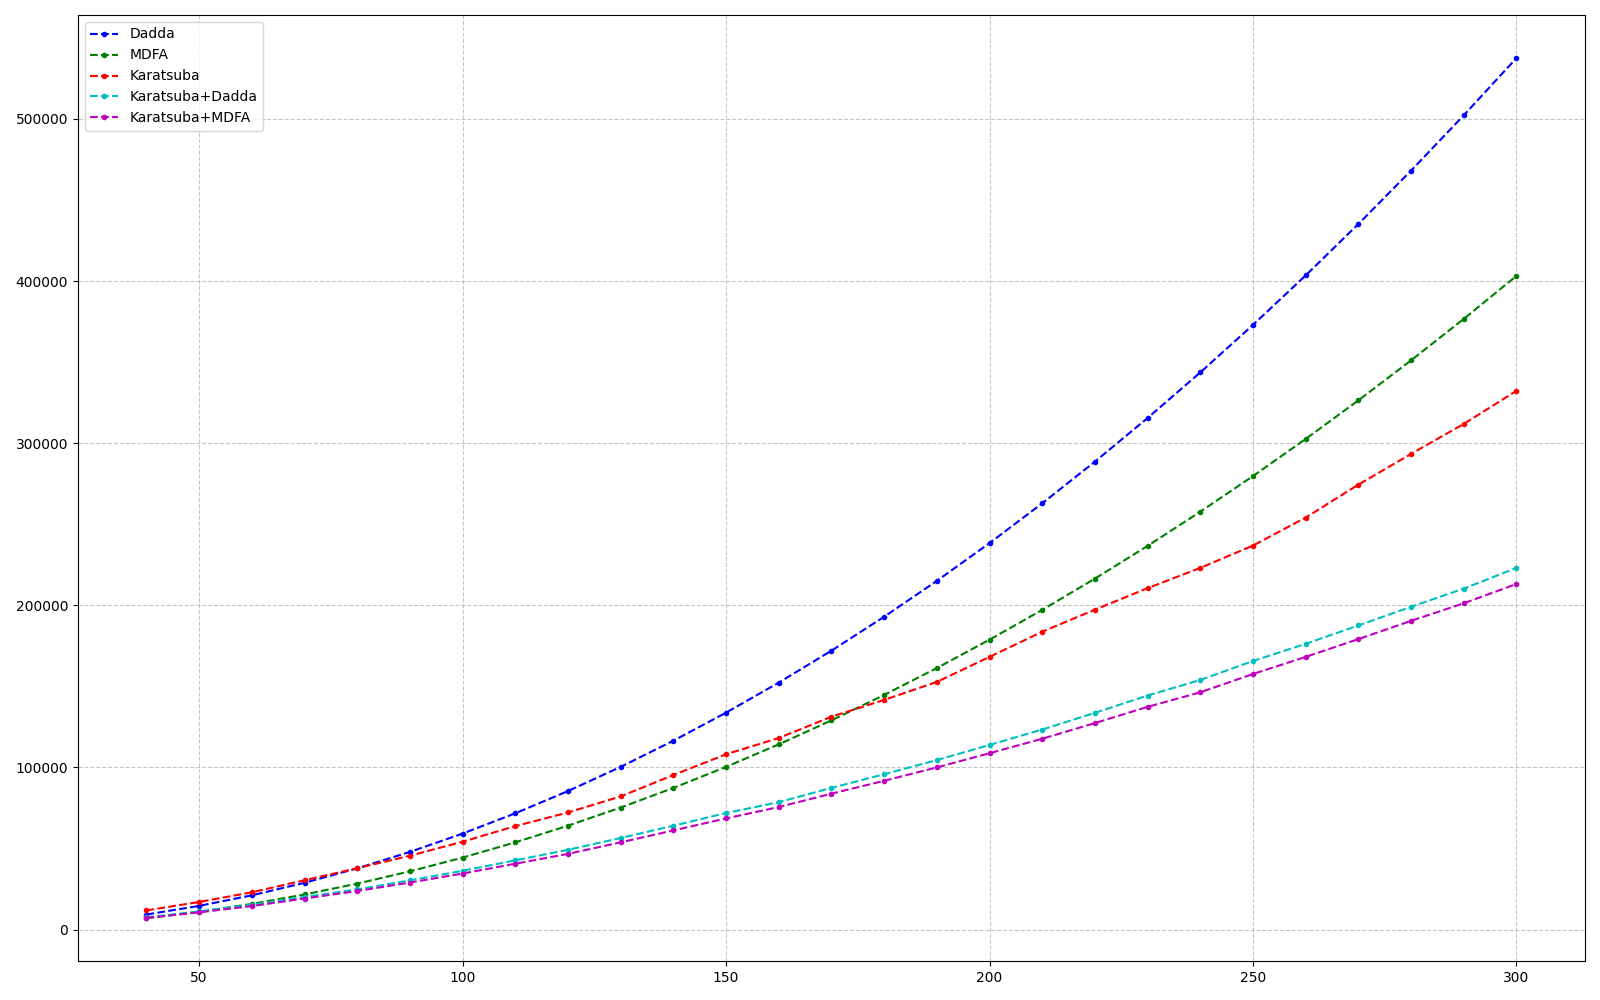
\includegraphics[width=\linewidth]{images/plot40_300_10}
        \caption{Comparing the size of~five circuit designs for $\MULT_n$, for $40 \le n \le 300$.}
        \label{figure:multiplication}
    \end{figure}

    \subsection{Logarithmic Depth}
    The depth of~most of~the circuits described above
    is~linear, that~is, $\Theta(n)$.
    With an~additional care, one can make the depth logarithmic ($\Theta(\log n)$) by~increasing the size slightly.
    To~achieve this, one processes the layers in~parallel rather than consecutively.
    Namely, let $h$~be the maximum height of~a~significance layer (that~is, every layer contains at~most $h$~bits). While $h > 3$, apply in~parallel as~many
    FA's as~possible to~every layer. After one such step, the maximum height becomes at~most $2h/3$ (to~simplify the exposition, we~ignore constant additive terms here): indeed, if~there are $k \le h$ bits on~the current layer, then about $k/3 \le h/3$ bits remain after the application of FA's; also, at~most $h/3$ bits are transferred from the next layer. Since the maximum height decreases geometrically, in~at most $O(\log n)$ steps, one reaches the case when $h \le 3$.
    This takes depth $O(\log n)$ and size $O(n)$ (since each FA reduces the total number of~bits by~one). When $h \le 3$, apply either HA~or~FA to~every layer. This ensures that every layer has at~most two bits, that~is, $h \le 2$ (the size of~the resulting circuit is~still linear and the depth is~still logarithmic).
    Then, everything boils down to~adding
    two $k$-bit numbers (with $k \le n$). This can
    be~performed using, for example,
    the Brent--Kung adder~\cite{BrentKung1982} that has size $O(k)$ and depth $O(\log k)$. By~using MDFA's instead of~FA's, one can further reduce the size of~the resulting circuits. Table~\ref{table:log} shows the size and the depth of the circuits generated this way for the three previously considered functions: $\SUM$, $\ADD$, and $\MULT$.

	\begin{table*}[ht]
		\caption{The size and the depth of~circuits computing $\SUM_n$, $\ADD_n$, and $\MULT_n$.}
		\label{table:log}
		\begin{center}
			\begin{tabular}{{lrrrrrrrrl}}
				\toprule
				$n$ & 10 & 20 & 30 & 40 & 60 & 80 & 160 & 320 \\
				\midrule
				\multirow{2}{*}{ADD}  & 15 & 18	& 23 & 24 & 28 & 31 & 32 & 42 & depth \\
				& 49 & 101 & 153 & 194 & 297 & 383 & 755 & 1526 & size \\
				\midrule
				\multirow{2}{*}{SUM}  & 10 & 14 & 16 & 18 & 20 & 22 & 26 & 30 & depth \\
				& 64 & 141 & 215 & 298 & 452 & 615 & 1252 & 2529 & size \\
				\midrule
				\multirow{2}{*}{MULT} & 28 & 38 & 45 & 50 & 54 & 61 & 69 & 80 & depth \\
				& 527 & 1901 & 4309 & 7558 & 16756 & 29571 & 116788 & 464139 & size \\
				\bottomrule
			\end{tabular}
		\end{center}
	\end{table*}




    \section{Conclusion and Further Directions}
    In this paper, we~presented smaller circuits for bit addition.
    In~many practically relevant scenarios, the described circuits
    are about 10\% smaller than the known circuits composed
    out~of Half Adders and Full Adders.
    Also, we~implemented generators that allow one
    to~produce the corresponding circuits using a~single line of~code
    via the \texttt{Cirbo} open-source package~\cite{DBLP:conf/aaai/AverkovBEGKKKLL25}.

    %\subsection{Better Size Upper Bounds}
    There are three natural open problems related to~the circuit size of~bit addition.
    \begin{enumerate}
        \item What is the largest $\alpha$ such that
        \[\size(\BA_n^s) \le 4.5n-\alpha m\]
        holds for every vector~$s$? In~this paper, we~proved that $\alpha \ge 2$.
        Theorem~\ref{theorem:main} shows that $\alpha \le 2.5$. An~example
        of~a~vector where our upper bound $4.5n-2m$ matches the size of~the circuit
        produced by~our algorithm~is
        \[s^*=\left(0,0,0,0,1,1,2,2,\dotsc,\frac{n}{2}-2, \frac{n}{2}-2\right).\]
        \begin{center}
            \begin{tikzpicture}
                \foreach \x [count=\n from 0] in {2, 1, ..., -6} {
                    \draw[l] (\x * \d, -1) -- (\x * \d, 0.75);
                    \node[below] at (\x * \d, -1) {$\n$};
                }

                \foreach \x in {-6, ..., 2} {
                    \node[dot] at (\x * \d, - 2 * \d) {};
                    \node[dot] at (\x * \d, - \d) {};
                }
                \node[dot] at (2 * \d, 0) {};
                \node[dot] at (2 * \d, \d) {};
            \end{tikzpicture}
        \end{center}
        In~this case, our method first spends $n/2$ gates to~pair the bits and then applies $n/2$ MDFA' blocks. The size of~the resulting circuit~is, up~to an~additive constant, $n/2+6\cdot n/2=3.5n$. This matches the upper bound $4.5n-2m$. Thus, to~improve the bound $4.5n-2m$ to~$4.5n-\beta m$, for $\beta > 2$, one needs to~find a~smaller circuit for this particular vector~$s^*$.
        And vice versa, by~proving a~lower bound $\size(\BA_n^{s^*}) \ge 3.5n-O(1)$,
        one would prove that $\alpha=2$.

        \item What is the smallest $\gamma$ such that
        \[\size(\BA_n^s) \le \gamma n-O(m)\]
        holds for every vector~$s$? In~this paper,
        we~proved that $\gamma \le 4.5$.
        Improving this seems to~be more challenging than just improving $2m$~to~$2.5m$ as~this would most probably require using new building blocks.

        \item Finally, note also that the upper bounds $5n-3m$ and $4.5n-2m$ hold for \emph{all} vectors~$s$.
        It~would be~interesting to~improve known upper and lower bounds for \emph{specific} vectors. Perhaps, one of~the most interesting such functions is~$\SUM_n$ (here, $s=(0,0,\dotsc,0)$). For~it, we~known an~upper bound $4.5n$ (originally proved
        by~Demenkov et al.~\cite{DBLP:journals/ipl/DemenkovKKY10}; also follows from our Theorem~\ref{theorem:main}) and a~lower bound $2.5n-O(1)$ due to~Stockmeyer~\cite{DBLP:journals/mst/Stockmeyer77}.
    \end{enumerate}

    \section*{Acknowledgments}
    We~thank the anonymous reviewers for many helpful comments.

    \bibliography{references}
\end{document}
